\documentclass[12pt]{exam}
\printanswers
\usepackage[utf8]{inputenc}
\usepackage[a4paper, total={6in,4in}]{geometry}
\usepackage{geometry}
\usepackage{amsmath}
\usepackage{amssymb}
\geometry{left=2cm, right=2cm, top=2cm, bottom=2cm}
\usepackage{tikz}
\usepackage{tikz-qtree}
\usepackage{fixltx2e}
\usepackage{makecell}
\usetikzlibrary{automata, positioning, arrows}
\tikzset{
->, % makes the edges directed
>=stealth', % makes the arrow heads bold
node distance=3cm, % specifies the minimum distance between two nodes. Change if necessary.
every state/.style={thick}, % sets the properties for each ’state’ node
initial text=$ $, % sets the text that appears on the start arrow
}
\newcommand\scalemath[2]{\scalebox{#1}{\mbox{\ensuremath{\displaystyle #2}}}}



\title{
  Assignment 2\\
  \large CMPUT 474
}
\author{Pranav Wadhwa\\1629510}

\begin{document}
\maketitle
\noindent

\begin{questions}

  % Question 1
  \question{} Are the following languages context-free? Prove your answer in each case.
  \begin{parts}
    \part $\Sigma = \{0,1\}^{*}, L=\{xy \,|\,|x| = |y|, x\neq y\}$
    \part $\Sigma = \{0,1\}^{*}, L=\{w \,|\, n_{0}(w)=n_{1}(w) \text{ and } w \text{ includes the string '001'}\}$ where $n_{0}(w)$ and $n_{1}(w)$ denote the number of 0s and 1s in $w$ respectively.

    \begin{solution}
      Yes, the language is context free. We observe in language $L$ that it is made up of 2 strings $x$ and $y$ which are of same length but the strings are not equal. So the strings differ on some character $i$ and we can make a correcponding context-free grammar around this rule.

      \begin{gather*}
        S\to AB|BA\\
        A\to XAX|0\\
        B\to XBX|1\\
        X\to 0|1
      \end{gather*}


    \end{solution}


  \end{parts}

  % Question 2
  \question{} Let $G$ be a CFG in Chomsky normal form, and $w\in L(G)$. How long is $w$ if there is a derivation of $w$ using $p$ steps? Explain why.

  \begin{solution}

    Every context-free grammar that is in Comsky normal form has rules of the form
    \begin{gather*}
      A\to BC\\
      A\to a
    \end{gather*}
    We have $G$ a CGC in Chimsky normal form and $w\in L(G)$. $w$ is derivated in $p$ steps.
    Every derivattion in this form goes from $A\text{ (non-terminal)} \to BC\text{ (non-terminal)(non-terminal)}$ or $A\text{ (non-terminal)}\to a \text{ terminal }$.

    To derive a string of length $w$ we will have $w$ derivation of the first form from $A\to BC$ to a terminal $A\to a$ while expanding $B$ as each step adds a total of $+1$ to each step. Then we will have a total of $w-1$ derivation from $A\to C$ while expanding $C$ to a terminal as the start symbol is already counted.

    So the total number of derivations are $w + (w-1) = 2w-1$. We are given than the total derivations are $p$.

    So, $p = 2w-1$ then $w = \frac{p+1}{2}$


  \end{solution}

  % Question 3
  \question{} Let $G$ be a CFG. Explain an algorithm to determine whether $L(G)$ is finite. (Hint: use the pumping lemma).

  % question 4
  \question{} Convert the CFG
  \begin{gather*}
  S\to E\\
    E\to E+T|T\\
    T\to T \times F|F\\
    F\to (E)|\text{a}
    \end{gather*}
  to an equivalent PDA.

  \begin{solution}

    A GPDA of the CFC

    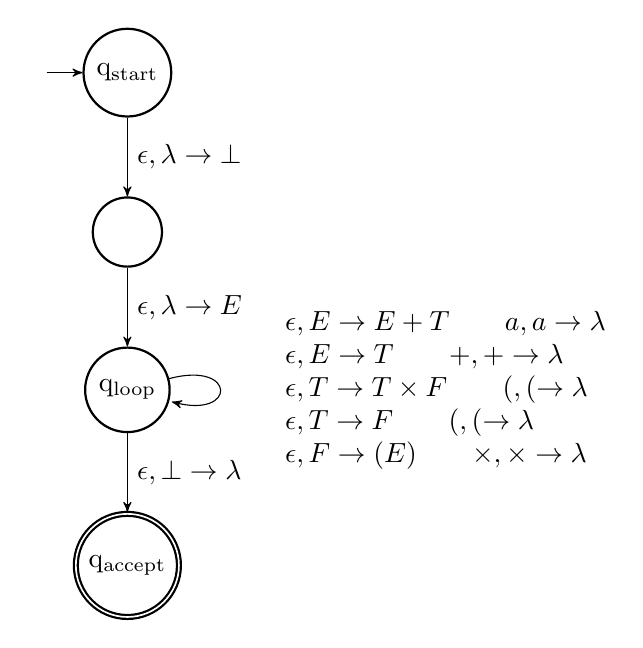
\begin{tikzpicture}
      \node[state, initial] (q1) {q\textsubscript{start}};
      \node[state, below=1cm of q1] (q12) {};
      \node[state, below=1cm of q12] (q2) {q\textsubscript{loop}};
      \node[state, below=1cm of q2, accepting] (q3) {q\textsubscript{accept}};


      \draw (q1) edge[right] node{$\epsilon, \lambda \to \bot$} (q12)
      (q12) edge[right] node{$\epsilon, \lambda \to E$} (q2)
      (q2) edge[right] node{$\epsilon, \bot \to \lambda$} (q3)
      (q2) edge[in=120, out=60,loop right=150] node[align=center]{\makecell[l]{$\qquad\epsilon, E\to E+T\qquad  a, a\to \lambda$\\
        $\qquad\epsilon, E\to T\qquad  +, +\to \lambda$\\$\qquad\epsilon, T\to T\times F\qquad (, (\to \lambda$\\$\qquad\epsilon, T\to F\qquad (, (\to \lambda$\\$\qquad\epsilon, F\to (E)\qquad \times, \times \to \lambda$}} (q2);
    \end{tikzpicture}

  \end{solution}


  % Question 5
  \question{} Recall that the class of context-free language is closed uner the regular operations, union, concatenation, and star. Prove that every regular language is context free by showing how to convert a regualar expression directly to an equivalent context-free grammar.


  % Question 6
  \question{} Consider the CFG G given by
  \[S\to \mathsf{a}S\mathsf{b}S\,|\,\mathsf{b}S\mathsf{a}S\,|\,\epsilon\]
  Prove that $L(G)$ is the set of strings with an equal number of $a$s and $b$s.

  \begin{solution}

    We want to show that every string s in $L(G)$ contains an equal number of a$s$ and b$s$ with strong induction.

    Base Case:\\
    $|s| = 1$. If s is generated by $G$ then the only possible string is $\epsilon$ which has $n_{a}= n_{b}=0$\\
    $|s| = 2$. If s is generated by $G$ then the possible string are $ab$ or $ba$ where both have $n_{a} = n_{b} = 1$.\\
    Inductive Hypothesis (IH):\\
    $G$ produces strings that have $n_{a} = n_{b}$ (number of a$s$ is equal to number of b$s$).\\
    Inductive Step:\\
    Assume that $IH$ holds for all strings in $G$ that have length $n$ or less than $n$. Consider the string $s$ of length $n+1$ and it is begin produces by rule S. We wil go over each rule and see how it is generated.\\
    If we use rule $S\to \mathsf{a}S\mathsf{b}S$ then $s$ consists of $\mathsf{a}w_{1}\mathsf{b}w_{2}$ where $w_{1}$ and $w_{2}$ are string derived from $G$ and are of length less than $n$. From our $IH$ we know than $w_{1}$ and $w_{2}$ have equal number of a$s$ and b$s$. So then length of string $|s| = |a| + |w_{1}| + |b| + |w_{2}|$ and string $s$ adds one pair of a,b to $w_{1}$ and $w_{2}$ which makes the total number of a$s$ and b$s$ in $s$ to be equal.\\
    Similarly, if we use the rule $S\to \mathsf{b}S\mathsf{a}S$ we find that it is made up of strings $\mathsf{b}w_{1}\mathsf{a}w_{2}$ where $w_{1}$ and $w_{2}$ are both derived from $G$ are are of length less than $n$. Due to similar reasons given above the string $s$ generated by this rule also have equal number of a$s$ and b$s$.\\
    And lastly, if we use the rule $S\to \epsilon$ then the string $s$ would be of length $n$ which given by IH has equal number of a$s$ and b$s$.\\
    Therefore we have proved that IH holds for string $n+1$ then $L(G)$ is the set of strings with equal number of a$s$ and b$s$.
  \end{solution}


  % question 7
  \question{}
  Show the following grammar is ambiguous by drawing parse trees. Find an unambiguous grammer for this language.
  \[S\to \mathsf{a}S\mathsf{b}\,|\, S\mathsf{b}\,|\,\epsilon\]

  \begin{solution}

    Take this string generated from the grammer and its corresponding parse tree.
    \[abb\]

    \begin{tikzpicture}
    [
edge from parent path =  {(\tikzparentnode\tikzparentanchor) .. controls +(0,-1) and +(0,1) .. (\tikzchildnode\tikzchildanchor)}
    ]
      \node (q0) {S}
      child {node {a}}
      child {node {S}
        child {node {Sb}
          child {node {$\epsilon$}}
          child {node{b}}
        }
      }
      child {node {b}};

      \node [right=10cm of q0] {S}
      child {node {S}
        child {node {a}}
        child {node {S}
          child {node {$\epsilon$}}
        }
        child {node {b}}
      }
      child {node {b}};
    \end{tikzpicture}

    Since the string has 2 parse trees therefore, the grammer is ambiguous.


  \end{solution}


  % Question 8
  \question{}
  Let $P$ be the language of all palindromes over $\{0,1\}$ containing equal numbers of 0s and 1s. Show that $P$ is not context free.

  \begin{solution}
    We assume that $P$ is a CFL and obtain a contradiction. Let $p$ be the pumping length for $P$ and select a string that is a palindrome and also contains equal numbers of $0s$ and $1s$. So let $s = 1^{p}0^{p}1^{p}0^{p}$ be the string that is also in $P$. We can shorten $s$ into $s = 1^{p}0^{2p}1^{p}$.\\
    By the pumping lemma we may choose $u, v, x, y, z$ such that $|vy| > 0$ and $|vxy| < p$. We can look over different cases of $v$ and $y$.\\
    case 1: $v$ and $y$ are in the middle and only consists of $0s$. Then $uxz$ would contain less $0s$ then $1s$ as $uxz = 1^{p}0^{2p-|vx|}1^{p}$ which in not in $P$.\\
    case 2: $v$ or $y$ contains $m>0$ amount of $0s$ and $n>0$ amount of $1s$ from one side of the string but no $1s$ from the other size. Then the corresponding string $uxz$ generated would have the following cases for both sides:\\
    \[1^{p-m}0^{2p-n-|y|}1^{p}\quad \text{or} \quad 1^{p}0^{2p-n-|v|}1^{p-m}\]
    Both of them don't form a palimdrome as number of $1s$ are not equal so $uxz \notin P$. Therefore we obtain a contradiction and $P$ is not context free.
  \end{solution}


  % Question 9
  \question{}
  The language $L=\{ww: w\in \{a,b\}^{*}\}$ is not context free. However, show that the complement language, $\bar{L}$, is context free.

  % Question 10
  \question{}
  Is there a \emph{universal} pusdown automaton? That is, there is a single pushdown automaton, say $M$ such that given a string $s_{G}w$, where $s_{g}$ is a string that describes a context free grammar and $w$ is an input string, $M$ accepts $s_{G}w$ if and only if $G$ generates $w$? Explain your answer.
\end{questions}

\end{document}
